\documentclass{ashoka-crypto}
\usepackage{enumitem, hyperref}
\graphicspath{ {images/} }

\author{Aryan Nath} % Your name
\problem{1} % Problem set number

\collab{none}
% or give names, e.g., \collab{Alyssa P. Hacker and A. Student}

\begin{document}

\section*{Problem 1 [5 points]}

\begin{figure}[h]
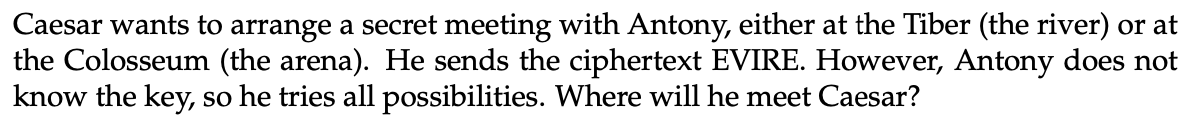
\includegraphics[width=17cm]{1}
\end{figure}

On using all possible keys, Antony gets both RIVER (K = 13) and ARENA (K = 22) as possible plaintexts. So he won't be able to make a decision on where to meet Caesar.

The set of possible decryptions are as follows:

\begin{table}[ht]
\centering
\begin{tabular}{|c|c|}
\hline
\textbf{Key} & \textbf{Decryption} \\ \hline
0  & EVIRE  \\ \hline
1  & FWJSF  \\ \hline
2  & GXKTG  \\ \hline
3  & HYLUH  \\ \hline
4  & IZMVI  \\ \hline
5  & JANWJ  \\ \hline
6  & KBOXK  \\ \hline
7  & LCPYL  \\ \hline
8  & MDQZM  \\ \hline
9  & NERAN  \\ \hline
10 & OFSBO  \\ \hline
11 & PGTCP  \\ \hline
12 & QHUDQ  \\ \hline
\textbf{13} & \textbf{RIVER}  \\ \hline
14 & SJWFS  \\ \hline
15 & TKXGT  \\ \hline
16 & ULYHU  \\ \hline
17 & VMZIV  \\ \hline
18 & WNAJW  \\ \hline
\end{tabular}
\end{table}

\begin{table}[ht]
\centering
\begin{tabular}{|c|c|}
\hline
\textbf{Key} & \textbf{Decryption} \\ \hline
19 & XOBKX  \\ \hline
20 & YPCLY  \\ \hline
21 & ZQDMZ  \\ \hline
\textbf{22} & \textbf{ARENA}  \\ \hline
23 & BSFOB  \\ \hline
24 & CTGPC  \\ \hline
25 & DUHQD  \\ \hline
\end{tabular}
\end{table}

\section*{Problem 2 [10 points]}

\begin{figure}[h]
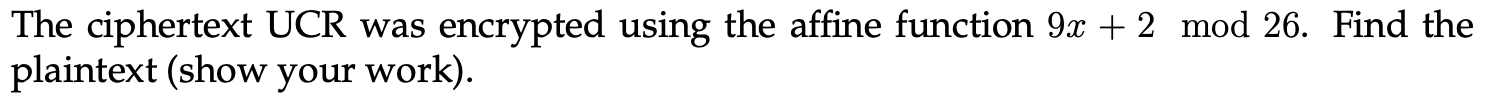
\includegraphics[width=17cm]{2}
\end{figure}

Use the ciphertext UCR, and assume the encryption is in the form of a stream cipher.\\\\
So first convert the ciphertext to a vector of integers = $<20, 2, 17>$.\\\\
Now feed each of these to the affine function:
\begin{enumerate}
\item $20 \rightarrow 9\times x + 2 \equiv 20 \pmod {26} \Rightarrow 9\times x \equiv 18 \pmod {26}$.\\
The inverse of $9 \pmod {26}$ is 3 [since $9\times 3 = 27 \equiv 1 \pmod {26}$].\\
$\Rightarrow 3\times 9 \times x \equiv 54 \pmod {26} \Rightarrow 1 \times x \equiv 2 \pmod {26}$\\
$\Rightarrow x = 2 \pmod {26}$
\item $2 \rightarrow 9 \times x + 2 \equiv 2 \pmod {26} \Rightarrow 9 \times x \equiv 0 \pmod {26}$\\
$\Rightarrow 3\times 9 \times x \equiv 0 \pmod {26}$\\
$\Rightarrow x = 0 \pmod {26}$
\item $17 \rightarrow 9 \times x + 2 \equiv 17 \pmod {26} \Rightarrow 9 \times x \equiv 15 \pmod {26}$\\
$\Rightarrow 3\times 9 \times x \equiv 45 \pmod {26} \Rightarrow 1 \times x \equiv 19 \pmod {26}$\\
$\Rightarrow x \equiv 19 \pmod {26}$.
\end{enumerate}

Hence, the obtained vector for the plaintext is $<2,0,19>$.\\
Converting these to ASCII characters using an offset of $65$ on each integer gives the plaintext as:\\
$<2,0,19> \rightarrow \textbf{CAT}$. 

\section*{Problem 3 [30 points]}

\begin{figure}[h]
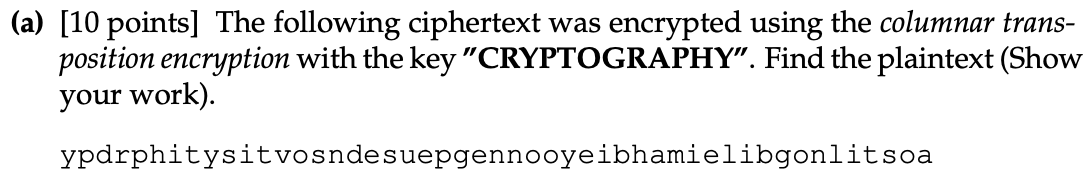
\includegraphics[width=17cm]{3a}
\end{figure}

Keeping the order of the key characters in "CRYPTOGRAPHY" in the transposition matrix, with the last row having the remainder of the ciphertext length by the key length, the ciphertext characters are added in the sorted order of the key characters to get back the plaintext:

\begin{center}
\begin{tabular}{|c|c|c|c|c|c|c|c|c|c|c|c|}
\hline
1          & 7          & 10         & 5          & 9          & 4          & 2          & 8          & 0          & 6          & 3          & 11         \\ \hline
\textbf{C} & \textbf{R} & \textbf{Y} & \textbf{P} & \textbf{T} & \textbf{O} & \textbf{G} & \textbf{R} & \textbf{A} & \textbf{P} & \textbf{H} & \textbf{Y} \\ \hline
           &            &            &            &            &            &            &            & y          &            &            &            \\ \hline
           &            &            &            &            &            &            &            & p          &            &            &            \\ \hline
           &            &            &            &            &            &            &            & d          &            &            &            \\ \hline
           &            &            &            &            &            &            &            & r          &            &            &            \\ \hline
           &     -       &    -        &      -     &     -       &      -      &     -       &     -       &      -      &     -       &       -     &  -            \\ \hline
\end{tabular}
\end{center}

\begin{center}
\begin{tabular}{|c|c|c|c|c|c|c|c|c|c|c|c|}
\hline
1          & 7          & 10         & 5          & 9          & 4          & 2          & 8          & 0          & 6          & 3          & 11         \\ \hline
\textbf{C} & \textbf{R} & \textbf{Y} & \textbf{P} & \textbf{T} & \textbf{O} & \textbf{G} & \textbf{R} & \textbf{A} & \textbf{P} & \textbf{H} & \textbf{Y} \\ \hline
p          &            &            &            &            &            &            &            & y          &            &            &            \\ \hline
h          &            &            &            &            &            &            &            & p          &            &            &            \\ \hline
i          &            &            &            &            &            &            &            & d          &            &            &            \\ \hline
t          &            &            &            &            &            &            &            & r          &            &            &            \\ \hline
y         &     -       &    -        &      -     &     -       &      -      &     -       &     -       &      -      &     -       &       -     &  -            \\ \hline
\end{tabular}
\end{center}

\begin{center}
\begin{tabular}{|c|c|c|c|c|c|c|c|c|c|c|c|}
\hline
1          & 7          & 10         & 5          & 9          & 4          & 2          & 8          & 0          & 6          & 3          & 11         \\ \hline
\textbf{C} & \textbf{R} & \textbf{Y} & \textbf{P} & \textbf{T} & \textbf{O} & \textbf{G} & \textbf{R} & \textbf{A} & \textbf{P} & \textbf{H} & \textbf{Y} \\ \hline
p          &            &            &            &            &            & s          &            & y          &            &            &            \\ \hline
h          &            &            &            &            &            & i          &            & p          &            &            &            \\ \hline
i          &            &            &            &            &            & t          &            & d          &            &            &            \\ \hline
t          &            &            &            &            &            & v          &            & r          &            &            &            \\ \hline
y          &     -       &    -        &      -     &     -       &      -      &     -       &     -       &      -      &     -       &       -     &  -            \\ \hline
\end{tabular}
\end{center}

\begin{center}
\begin{tabular}{|c|c|c|c|c|c|c|c|c|c|c|c|}
\hline
1          & 7          & 10         & 5          & 9          & 4          & 2          & 8          & 0          & 6          & 3          & 11         \\ \hline
\textbf{C} & \textbf{R} & \textbf{Y} & \textbf{P} & \textbf{T} & \textbf{O} & \textbf{G} & \textbf{R} & \textbf{A} & \textbf{P} & \textbf{H} & \textbf{Y} \\ \hline
p          &            &            &            &            &            & s          &            & y          &            & o          &            \\ \hline
h          &            &            &            &            &            & i          &            & p          &            & s          &            \\ \hline
i          &            &            &            &            &            & t          &            & d          &            & n          &            \\ \hline
t          &            &            &            &            &            & v          &            & r          &            & d          &            \\ \hline
y          &     -       &    -        &      -     &     -       &      -      &     -       &     -       &      -      &     -       &       -     &  -            \\ \hline
\end{tabular}
\end{center}

\begin{center}
\begin{tabular}{|c|c|c|c|c|c|c|c|c|c|c|c|}
\hline
1          & 7          & 10         & 5          & 9          & 4          & 2          & 8          & 0          & 6          & 3          & 11         \\ \hline
\textbf{C} & \textbf{R} & \textbf{Y} & \textbf{P} & \textbf{T} & \textbf{O} & \textbf{G} & \textbf{R} & \textbf{A} & \textbf{P} & \textbf{H} & \textbf{Y} \\ \hline
p          &            &            &            &            & e          & s          &            & y          &            & o          &            \\ \hline
h          &            &            &            &            & s          & i          &            & p          &            & s          &            \\ \hline
i          &            &            &            &            & u          & t          &            & d          &            & n          &            \\ \hline
t          &            &            &            &            & e          & v          &            & r          &            & d          &            \\ \hline
y          &     -       &    -        &      -     &     -       &      -      &     -       &     -       &      -      &     -       &       -     &  -            \\ \hline
\end{tabular}
\end{center}

\begin{center}
\begin{tabular}{|c|c|c|c|c|c|c|c|c|c|c|c|}
\hline
1          & 7          & 10         & 5          & 9          & 4          & 2          & 8          & 0          & 6          & 3          & 11         \\ \hline
\textbf{C} & \textbf{R} & \textbf{Y} & \textbf{P} & \textbf{T} & \textbf{O} & \textbf{G} & \textbf{R} & \textbf{A} & \textbf{P} & \textbf{H} & \textbf{Y} \\ \hline
p          &            &            & p          &            & e          & s          &            & y          &            & o          &            \\ \hline
h          &            &            & g          &            & s          & i          &            & p          &            & s          &            \\ \hline
i          &            &            & e          &            & u          & t          &            & d          &            & n          &            \\ \hline
t          &            &            & n          &            & e          & v          &            & r          &            & d          &            \\ \hline
y          &     -       &    -        &      -     &     -       &      -      &     -       &     -       &      -      &     -       &       -     &  -            \\ \hline
\end{tabular}
\end{center}

\begin{center}
\begin{tabular}{|c|c|c|c|c|c|c|c|c|c|c|c|}
\hline
1          & 7          & 10         & 5          & 9          & 4          & 2          & 8          & 0          & 6          & 3          & 11         \\ \hline
\textbf{C} & \textbf{R} & \textbf{Y} & \textbf{P} & \textbf{T} & \textbf{O} & \textbf{G} & \textbf{R} & \textbf{A} & \textbf{P} & \textbf{H} & \textbf{Y} \\ \hline
p          &            &            & p          &            & e          & s          &            & y          & n          & o          &            \\ \hline
h          &            &            & g          &            & s          & i          &            & p          & o          & s          &            \\ \hline
i          &            &            & e          &            & u          & t          &            & d          & o          & n          &            \\ \hline
t          &            &            & n          &            & e          & v          &            & r          & y          & d          &            \\ \hline
y          &     -       &    -        &      -     &     -       &      -      &     -       &     -       &      -      &     -       &       -     &  -            \\ \hline
\end{tabular}
\end{center}

\begin{center}
\begin{tabular}{|c|c|c|c|c|c|c|c|c|c|c|c|}
\hline
1          & 7          & 10         & 5          & 9          & 4          & 2          & 8          & 0          & 6          & 3          & 11         \\ \hline
\textbf{C} & \textbf{R} & \textbf{Y} & \textbf{P} & \textbf{T} & \textbf{O} & \textbf{G} & \textbf{R} & \textbf{A} & \textbf{P} & \textbf{H} & \textbf{Y} \\ \hline
p          & e          &            & p          &            & e          & s          &            & y          & n          & o          &            \\ \hline
h          & i          &            & g          &            & s          & i          &            & p          & o          & s          &            \\ \hline
i          & b          &            & e          &            & u          & t          &            & d          & o          & n          &            \\ \hline
t          & h          &            & n          &            & e          & v          &            & r          & y          & d          &            \\ \hline
y          &     -       &    -        &      -     &     -       &      -      &     -       &     -       &      -      &     -       &       -     &  -            \\ \hline
\end{tabular}
\end{center}

\begin{center}
\begin{tabular}{|c|c|c|c|c|c|c|c|c|c|c|c|}
\hline
1          & 7          & 10         & 5          & 9          & 4          & 2          & 8          & 0          & 6          & 3          & 11         \\ \hline
\textbf{C} & \textbf{R} & \textbf{Y} & \textbf{P} & \textbf{T} & \textbf{O} & \textbf{G} & \textbf{R} & \textbf{A} & \textbf{P} & \textbf{H} & \textbf{Y} \\ \hline
p          & e          &            & p          &            & e          & s          & a          & y          & n          & o          &            \\ \hline
h          & i          &            & g          &            & s          & i          & m          & p          & o          & s          &            \\ \hline
i          & b          &            & e          &            & u          & t          & i          & d          & o          & n          &            \\ \hline
t          & h          &            & n          &            & e          & v          & e          & r          & y          & d          &            \\ \hline
y          &     -       &    -        &      -     &     -       &      -      &     -       &     -       &      -      &     -       &       -     &  -            \\ \hline
\end{tabular}
\end{center}

\begin{center}
\begin{tabular}{|c|c|c|c|c|c|c|c|c|c|c|c|}
\hline
1          & 7          & 10         & 5          & 9          & 4          & 2          & 8          & 0          & 6          & 3          & 11         \\ \hline
\textbf{C} & \textbf{R} & \textbf{Y} & \textbf{P} & \textbf{T} & \textbf{O} & \textbf{G} & \textbf{R} & \textbf{A} & \textbf{P} & \textbf{H} & \textbf{Y} \\ \hline
p          & e          &            & p          & l          & e          & s          & a          & y          & n          & o          &            \\ \hline
h          & i          &            & g          & i          & s          & i          & m          & p          & o          & s          &            \\ \hline
i          & b          &            & e          & b          & u          & t          & i          & d          & o          & n          &            \\ \hline
t          & h          &            & n          & g          & e          & v          & e          & r          & y          & d          &            \\ \hline
y          &     -       &    -        &      -     &     -       &      -      &     -       &     -       &      -      &     -       &       -     &  -            \\ \hline
\end{tabular}
\end{center}

\begin{center}
\begin{tabular}{|c|c|c|c|c|c|c|c|c|c|c|c|}
\hline
1          & 7          & 10         & 5          & 9          & 4          & 2          & 8          & 0          & 6          & 3          & 11         \\ \hline
\textbf{C} & \textbf{R} & \textbf{Y} & \textbf{P} & \textbf{T} & \textbf{O} & \textbf{G} & \textbf{R} & \textbf{A} & \textbf{P} & \textbf{H} & \textbf{Y} \\ \hline
p          & e          & o          & p          & l          & e          & s          & a          & y          & n          & o          &            \\ \hline
h          & i          & n          & g          & i          & s          & i          & m          & p          & o          & s          &            \\ \hline
i          & b          & l          & e          & b          & u          & t          & i          & d          & o          & n          &            \\ \hline
t          & h          & i          & n         & g          & e          & v          & e          & r          & y          & d          &            \\ \hline
y          &     -       &    -        &      -     &     -       &      -      &     -       &     -       &      -      &     -       &       -     &  -            \\ \hline
\end{tabular}
\end{center}

\begin{center}
\begin{tabular}{|c|c|c|c|c|c|c|c|c|c|c|c|}
\hline
1          & 7          & 10         & 5          & 9          & 4          & 2          & 8          & 0          & 6          & 3          & 11         \\ \hline
\textbf{C} & \textbf{R} & \textbf{Y} & \textbf{P} & \textbf{T} & \textbf{O} & \textbf{G} & \textbf{R} & \textbf{A} & \textbf{P} & \textbf{H} & \textbf{Y} \\ \hline
p          & e          & o          & p          & l          & e          & s          & a          & y          & n          & o          & t          \\ \hline
h          & i          & n          & g          & i          & s          & i          & m          & p          & o          & s          & s          \\ \hline
i          & b          & l          & e          & b          & u          & t          & i          & d          & o          & n          & o          \\ \hline
t          & h          & i          & n          & g          & e          & v          & e          & r          & y          & d          & a          \\ \hline
y          &     -       &    -        &      -     &     -       &      -      &     -       &     -       &      -      &     -       &       -     &  -          \\ \hline
\end{tabular}
\end{center}

Reading row-wise, the obtained plaintext is:

"peoplesaynothingisimpossiblebutidonothingeveryday".

\clearpage 

\begin{figure}[h]
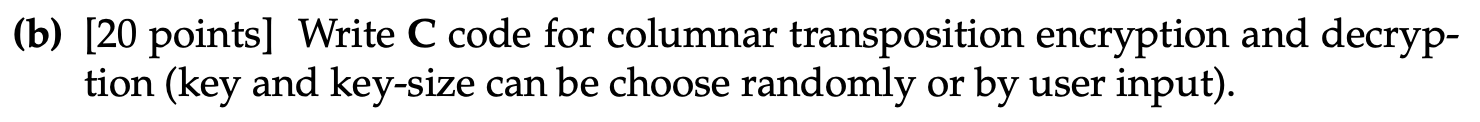
\includegraphics[width=17cm]{3b}
\end{figure}

Link to the file:

\href{https://drive.google.com/drive/folders/1tfEhPT_h7C7xW9Ym2BqReQu5e4RkwfLP?usp=sharing}{Question 3b}

Output:

Enter the key: CRYPTOGRAPHY\\
Enter the text: peoplesaynothingisimpossiblebutidonothingeveryday\\
Original text: peoplesaynothingisimpossiblebutidonothingeveryday\\
Encrypted text: ypdrphitysitvosndesuepgennooyamieeibhlibgonlitsoa\\
Decrypted text: peoplesaynothingisimpossiblebutidonothingeveryday\\

(Also submitted on google classroom)

\section*{Problem 4 [20 points]}

\begin{figure}[h]
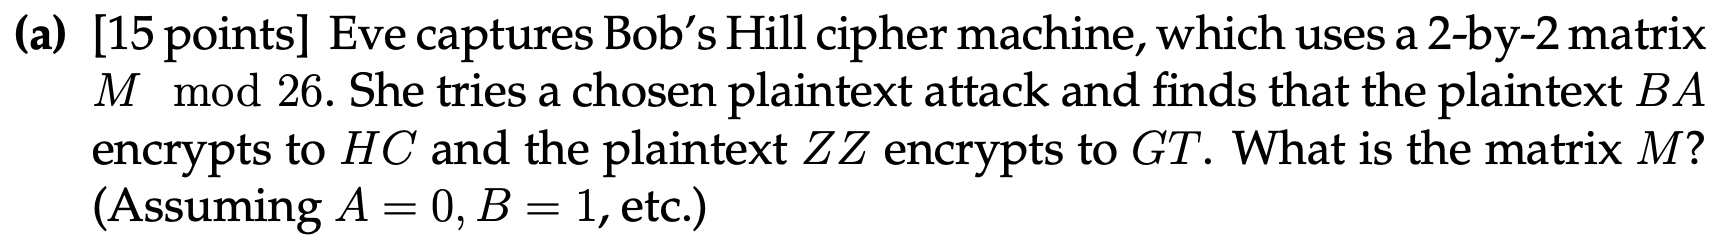
\includegraphics[width=17cm]{4a}
\end{figure}

%AA = 00, BA = 10

Let the matrix $M = 
\begin{bmatrix}
a & b \\
c & d
\end{bmatrix}$.\\

$\Rightarrow \begin{bmatrix}
a & b \\
c & d
\end{bmatrix}\begin{bmatrix}
1 \\
0
\end{bmatrix} = \begin{bmatrix}
7\\
2
\end{bmatrix} \pmod {26}$\\

and $\begin{bmatrix}
a & b \\
c & d
\end{bmatrix}\begin{bmatrix}
25 \\
25
\end{bmatrix} = \begin{bmatrix}
6\\
19
\end{bmatrix} \pmod {26}$

This gives us the following system of linear equations:
\begin{equation}
a = 7 \pmod {26}
\end{equation}
\begin{equation}
c = 2 \pmod {26}
\end{equation}
\begin{equation}
25a + 25b = 6 \pmod {26}
\end{equation}
\begin{equation}
25c + 25d = 19 \pmod {26}
\end{equation}

$\Rightarrow b = (6 - 175)*25^{-1} \pmod {26} = (-169)*25 \pmod {26} = 169 \pmod 26 = 13 \pmod {26}$\\
and $d = (19 - 50)*25^{-1} \pmod {26} = (-31)*25 \pmod{26} = 31 \pmod {26} = 5 \pmod {26}$

$\Rightarrow$ the matrix $M = \begin{bmatrix}
7 & 13\\
2 & 5
\end{bmatrix}$

\begin{figure}[h]
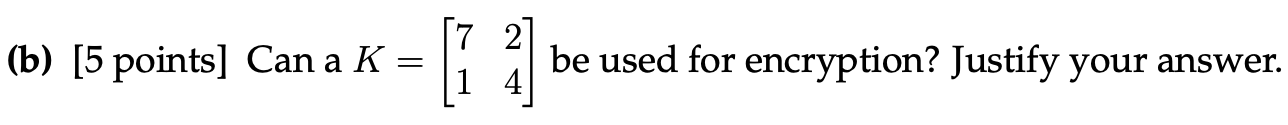
\includegraphics[width=17cm]{4b}
\end{figure}

No, this matrix cannot be used as the key. The determinant of $K$ is $26$, which is $0 \pmod{26}$. Hence, the inverse of the determinant does not exist in$\pmod{26}$. For decryption, the key matrix has to be inverted in $\pmod {26}$, since the determinant cannot be inverted, the matrix inverse cannot be calculated and decryption won't be possible with this matrix as the key.

\section*{Problem 5 [30 points]}

\begin{figure}[h]
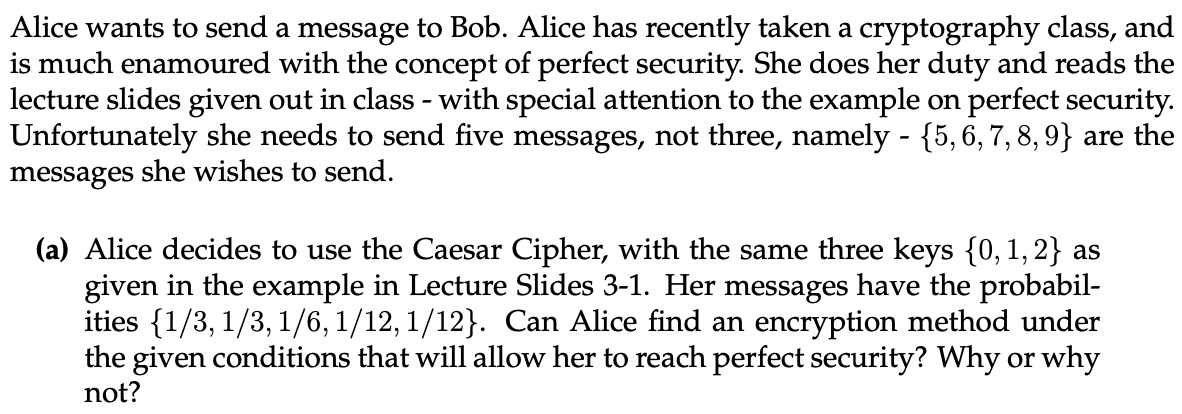
\includegraphics[width=17cm]{5a}
\end{figure}

We have been given the priori probabilities for message space. We can use the caesar cipher in modulo $5$ to each message uniquely:

$5 \rightarrow 0$\\
$6 \rightarrow 1$\\
$7 \rightarrow 2$\\
$8 \rightarrow 3$\\
$9 \rightarrow 4$

Assuming the key space is uniformly distributed, the probability distribution table can be constructed as follows,

\begin{table}[h]
\begin{tabular}{|c|ccc|}
\hline
  & 0    & 1    & 2    \\
  \hline
0 & 1/9  & 1/9  & 1/9  \\
1 & 1/9  & 1/9  & 1/9  \\
2 & 1/18 & 1/18 & 1/18 \\
3 & 1/36 & 1/36 & 1/36 \\
4 & 1/36 & 1/36 & 1/36\\
\hline
\end{tabular}
\centering
\end{table}

The (message, key, ciphertext) triplets can be constructed as follows:

\begin{table}[h]
\begin{tabular}{ccc}
(0,0,0)  & (0,1,1)  & (0,2,2)  \\
(1,0,1) & (1,1,2)  & (1,2,3)  \\
(2,0,2) & (2,1,3) & (2,2,4) \\
(3,0,3) & (3,1,4) & (3,2,0) \\
(4,0,4) & (4,1,0) & (4,2,1) \\
\end{tabular}
\centering
\end{table}

Now suppose the adversary receives the ciphertext $1$. The prior probability of the plaintext $4 (\text{or} \> 9)$ is $1/12$, i.e $P[m = 9] = 1/12$

Now, given the ciphertext $1$, the probability of getting $4 (\text{or} \> 9)$ as the plaintext can be calculated as follows:

\begin{math}
P[m=4|c=1] = \frac{P[m=4\land c=1]}{P[c=1]} = \frac{1/15}{1/9 + 1/9 + 1/36} = \frac{1/15}{9/36} = 4/15 \approx 0.266 \\
\end{math}

Comparing with the probability of randomly guessing the plaintext,

\begin{math}
P[m=4|c=1] \approx 0.266 > P[m = 4] = 1/12 \approx 0.083
\end{math}

So, when the adversary has the ciphertext $1$, they have a much higher probability $(0.266)$ of guessing the plaintext $1$ than when randomly guessing it with probability $1/12$.

Due to the smaller key space, the definition of perfect secrecy is not satisfied.

\begin{math}
P[m = m_0|c = c_0] = P[m = m_0]
\end{math}

is not met by Alice's encryption system.

\clearpage

\begin{figure}[h]
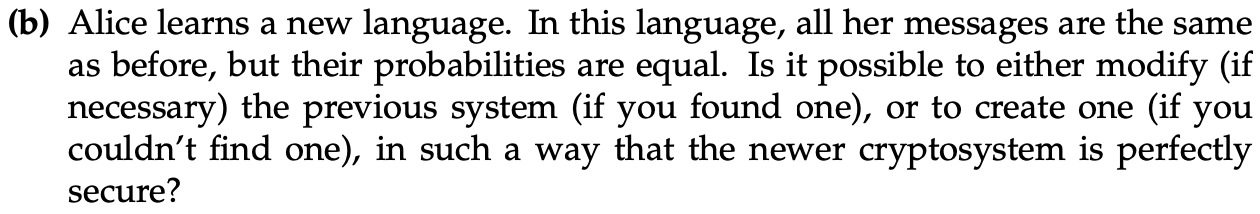
\includegraphics[width=17cm]{5b}
\end{figure}

The previous system can be modified to make it perfectly secure by increasing the key space to be equal to the size of the message space.

So, if the messages are $0,1,2,3,4 \pmod {5}$, the key space will be $0,1,2,3,4 \pmod {5}$.

Assuming the key space is uniformly distributed, the probability distribution table can be constructed as follows,


\begin{table}[h]
\begin{tabular}{|c|ccccc|}
\hline
  & 0    & 1    & 2 & 3 & 4   \\
  \hline
0 & 1/25  & 1/25  & 1/25 & 1/25 & 1/25  \\
1 & 1/25  & 1/25  & 1/25 & 1/25 & 1/25  \\
2 & 1/25  & 1/25  & 1/25 & 1/25 & 1/25 \\
3 & 1/25  & 1/25  & 1/25 & 1/25 & 1/25 \\
4 & 1/25  & 1/25  & 1/25 & 1/25 & 1/25 \\
\hline
\end{tabular}
\centering
\end{table}

The (message, key, ciphertext) triplet matrix will become:

\begin{table}[h]
\begin{tabular}{ccccc}
(0,0,0)  & (0,1,1)  & (0,2,2) & (0,3,3) & (0,4,4)  \\
(1,0,1) & (1,1,2)  & (1,2,3) & (1,3,4) & (1,4,0)  \\
(2,0,2) & (2,1,3) & (2,2,4) & (2,3,0) & (2,4,1) \\
(3,0,3) & (3,1,4) & (3,2,0) & (3,3,1) & (3,4,2) \\
(4,0,4) & (4,1,0) & (4,2,1) & (4,3,2) & (4,4,3) \\
\end{tabular}
\centering
\end{table}

Now each row (each plaintext) has each of the $5$ ciphertexts as its possible encryption. So knowing the ciphertext will not give the adversary any additional information about the plaintext. This can be expressed more strongly as,

\begin{math}
P[m = m_0 | c = c_0] = \frac{P[m = m_0 \land c = c_0]}{P[c = c_0]} = \frac{1/25}{5/25} = 1/5 = P[m = m_0]
\end{math}

for any $m_0$ and $c_0$ in $\pmod 5$.

Hence, this modified cryptosystem for Caesar cipher encryption is perfectly secure by definition of perfect secrecy.

\begin{figure}[h]
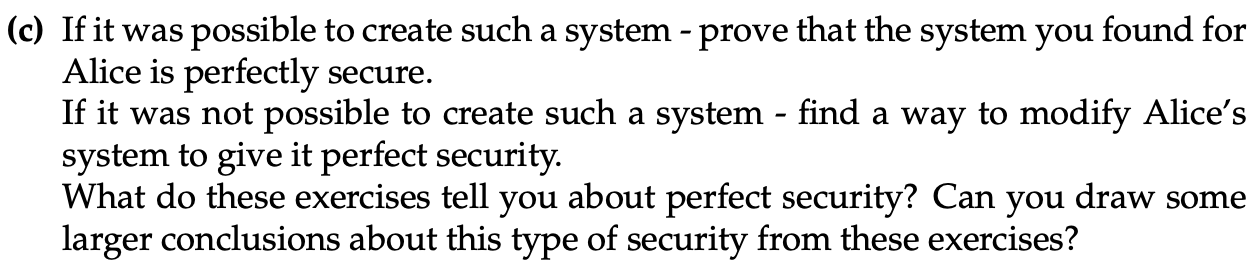
\includegraphics[width=17cm]{5c}
\end{figure}

Given that each message has probability $1/5$ in $\pmod 5$ and each key selection has probability $1/5$, the join probability distribution of the message space and the key space, 

\begin{table}[h]
\begin{tabular}{|c|ccccc|}
\hline
  & 0    & 1    & 2 & 3 & 4   \\
  \hline
0 & 1/25  & 1/25  & 1/25 & 1/25 & 1/25  \\
1 & 1/25  & 1/25  & 1/25 & 1/25 & 1/25  \\
2 & 1/25  & 1/25  & 1/25 & 1/25 & 1/25 \\
3 & 1/25  & 1/25  & 1/25 & 1/25 & 1/25 \\
4 & 1/25  & 1/25  & 1/25 & 1/25 & 1/25 \\
\hline
\end{tabular}
\centering
\end{table}

The (message, key, ciphertext) triplets in this cryptosystem become:

\begin{table}[h]
\begin{tabular}{ccccc}
(0,0,0)  & (0,1,1)  & (0,2,2) & (0,3,3) & (0,4,4)  \\
(1,0,1) & (1,1,2)  & (1,2,3) & (1,3,4) & (1,4,0)  \\
(2,0,2) & (2,1,3) & (2,2,4) & (2,3,0) & (2,4,1) \\
(3,0,3) & (3,1,4) & (3,2,0) & (3,3,1) & (3,4,2) \\
(4,0,4) & (4,1,0) & (4,2,1) & (4,3,2) & (4,4,3) \\
\end{tabular}
\centering
\end{table}

So for any plaintext $m_0$ and any ciphertext $c_0$, the conditional probability of guessing $m_0$ given $c_0$ is as follows,

\begin{math}
P[m = m_0 | c = c_0] = \frac{P[m = m_0 \land c = c_0]}{P[c = c_0]} = \frac{1/25}{5/25} = 1/5 = P[m = m_0]
\end{math}

The probability $P[m = m_0 | c = c_0]$ is equal to $1/12$ as each unique message ciphertext form a unique element in the triplet matrix, that is no two different encrypt $m_0$ to $c_0$.

Since the probability of guessing the plaintext when ciphertext is known is exactly the same as the probability of randomly guessing the ciphertext, the modifed cryptosystem for Alice's Caesar cipher encryption is perfectly secure.

These exercises tell me that perfect secrecy is affected by the size of the message space and the key space, even when the same encryption function is being used. Some larger conclusions that can be drawn are that, in order to have perfect secrecy the key space needs to be at least as large as the message space and that complete distribution of the ciphertext space (message space) over the set of possible encryptions for each message will ensure perfect secrecy.

\clearpage

\section*{Problem 6 [15 points]}

\begin{figure}[h]
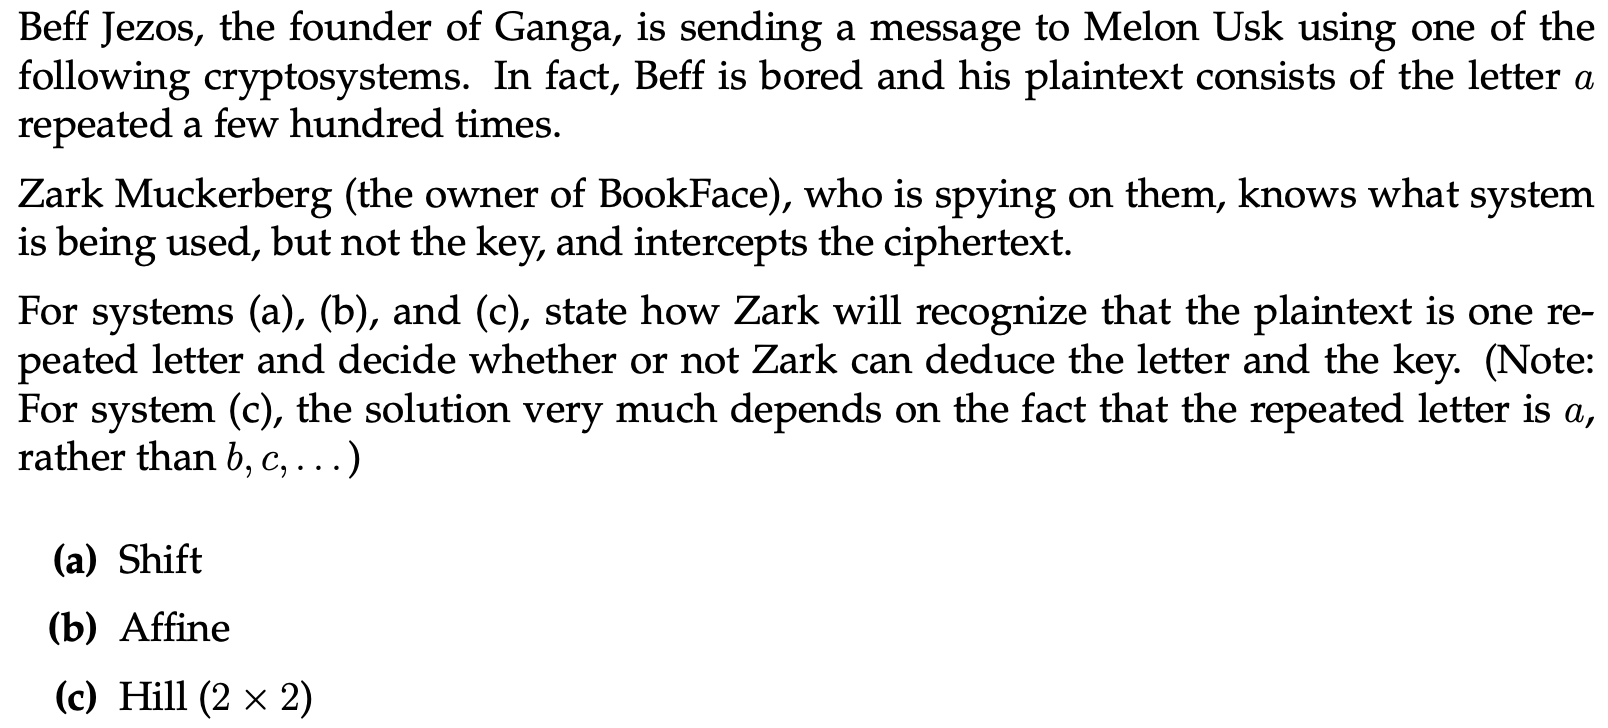
\includegraphics[width=17cm]{6}
\end{figure}

\begin{enumerate}[label=(\alph*)]
\item Shift Cipher:
Shifting of letter in this cipher is a one to one operation. So all repeated $a$'s will be mapped to the same letter. So for this case it will be simple for Zark to recognize that the plaintext is one repeated letter as all letters of the ciphertext will be the same. However, since the plaintext has no meaning, Zark cannot perform a letter frequency based attack or brute force attack to get the repeated letters of the plaintext as the plaintext is not representative of the letter distribution expected in an english paragraph. So the key can be any of $0,1,2,3,\dots,25$ and the repeated letter can be any of $a,b,c,\dots,z$ and Zark will not be able to deduce it.
\item Since the affine cipher is also a one to one function, Zark will recognize that the plaintext is one repeated character as all letters of the ciphertext will be the same. However, Zark will not be able to deduce the plaintext and the key through a brute force or frequency analysis attack, this is explained by the following example,

\begin{math}
3 \times x + 5 \equiv 0 \pmod{26} \Rightarrow x \equiv 7 \pmod {26}
\end{math}

But the encryption function can also be,

\begin{math}
3 \times x + 4 \equiv 0 \pmod{26} \Rightarrow x \equiv 16 \pmod {26}
\end{math}

So the plaintext can be $hhh\dots h$ or $qqq\dots q$, Zark won't be able to figure out which plaintext and key $(a,b)$ is correct as neither of these plaintexts has meaning comparable to an english paragraph.

\item Suppose the plaintext is $aa \dots a$. For encryption with a $2 \times 2$ matrix in a Hill cipher system, the plaintext is broken into pairs of two and multiplied with the key

$K = \begin{pmatrix}
a & b \\
c & d
\end{pmatrix}$ for $(a,b,c,d \in Z_{26})$ to get the ciphertext for each pair as,

\begin{center}
\begin{math}
\begin{pmatrix}
a & b \\
c & d
\end{pmatrix}
\begin{pmatrix}
0\\
0
\end{pmatrix}
\equiv 
\begin{pmatrix}
0\\
0
\end{pmatrix}
\pmod{26}
\end{math}
\end{center}

The ciphertex for $aa\dots a$ will be $00\dots 0$. Let $\alpha$ represent the integer modulo equivalent of any letter chosen other than $a$. Suppose the received ciphertext is still $00\dots 0$

\begin{center}
\begin{math}
\begin{pmatrix}
a & b \\
c & d
\end{pmatrix}
\begin{pmatrix}
\alpha \\
\alpha
\end{pmatrix}
\equiv 
\begin{pmatrix}
0\\
0
\end{pmatrix}
\pmod{26}
\end{math}
\end{center}

This means that, $(a + b)\alpha \equiv 0 \pmod{26}$ and $(c + d)\alpha \equiv 0 \pmod {26}$. Since $\alpha \not\equiv 0 \pmod {26}$, we get 

\begin{equation}
(a + b) \equiv 0 \pmod{26}
\end{equation}
\begin{equation}
(c + d) \equiv 0 \pmod{26}
\end{equation}

This mean that such a key will map every plaintext to the ciphertext $00\dots 0$.

Now, from the above modular equivalence we get,

\begin{center}
$a \equiv (-b) \pmod {26}$ and $c \equiv (-d) \pmod$
\end{center}

Through compatibility with scaling, we get,

\begin{center}
$a\cdot c \equiv (-b)\cdot c \pmod{26} \equiv (-b)(-d) \pmod 26 \equiv b\cdot d \pmod {26}$

$\Rightarrow a\cdot c - b \cdot d \equiv 0 \pmod {26}$

$\Rightarrow det(K) \equiv 0 \pmod {26}$
\end{center}

So such a key will never be used for encryption in the hill cipher as decryption wont be possible with it.

An even simpler proof would be,

Consider distinct $\alpha, \beta \in Z_{26}$,

\begin{center}
\begin{math}
\begin{pmatrix}
\alpha\\
\alpha
\end{pmatrix}
\not\equiv 
\begin{pmatrix}
\beta\\
\beta
\end{pmatrix}
\pmod{26}
\end{math}

But in the encryption we have,

\begin{math}
\begin{pmatrix}
a & b \\
c & d
\end{pmatrix}
\begin{pmatrix}
\alpha \\
\alpha
\end{pmatrix}
\equiv 
\begin{pmatrix}
a & b \\
c & d
\end{pmatrix}
\begin{pmatrix}
\alpha \\
\alpha
\end{pmatrix}
\equiv 
\begin{pmatrix}
0 \\
0
\end{pmatrix}
\pmod{26}
\end{math}

If $K$ is invertible, which is required for decryption, we get,

\begin{math}
\begin{pmatrix}
\alpha \\
\alpha
\end{pmatrix}
\equiv 
\begin{pmatrix}
\beta \\
\beta
\end{pmatrix}
\pmod{26}
\end{math}

\end{center}

This is a contraction.

Hence, the only possible plaintext for the given ciphertext $00\dots 0$ can be $aa\dots a$ and Zark will be able to deduce that the plaintext consists of repeated characters which can only be $a$. However they won't be able to deduce the key as this result will hold for any key $K$.
\end{enumerate}

\section*{Problem 7 [20 points]}

\begin{figure}[h]
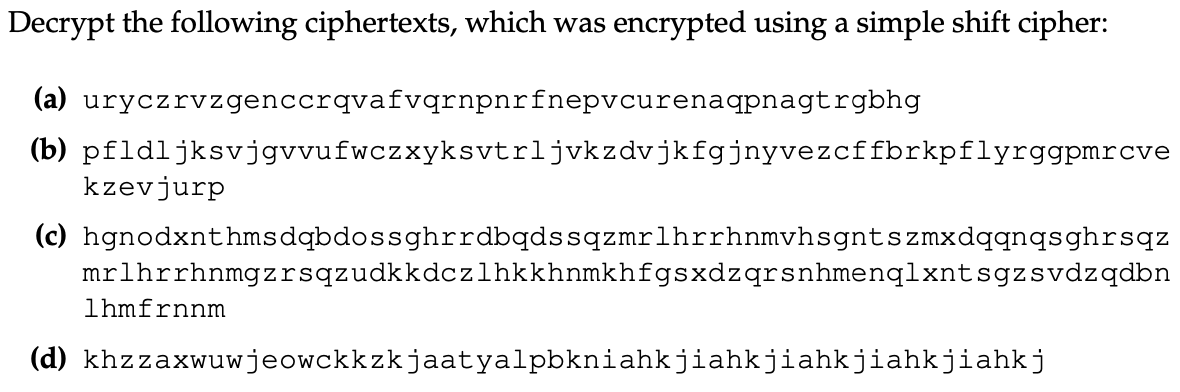
\includegraphics[width=17cm]{7}
\end{figure}

The ciphertexts can be decrypted using a brute force attack or using frequency analysis. I have used frequency analysis for the question.

To create the reference frequency table, I used text from the wikipedia pages of two of my favourite movies. The obtained frequency distribution is:

\[
\begin{array}{rcl}
0 & : & 0.09281588813456278, \\
1 & : & 0.015604417874151384, \\
2 & : & 0.03485662174485764, \\
3 & : & 0.03992299118451718, \\
4 & : & 0.11713446144492856, \\
5 & : & 0.02289998986726112, \\
6 & : & 0.018846894315533488, \\
7 & : & 0.04579997973452224, \\
8 & : & 0.07802208937075691, \\
9 & : & 0.0017225656094842436, \\
10 & : & 0.011247340156044179, \\
11 & : & 0.04529334279055629, \\
12 & : & 0.024622555476745363,
\end{array}
\]

\[
\begin{array}{rcl}
13 & : & 0.0738676664302361, \\
14 & : & 0.06576147532678082, \\
15 & : & 0.017326983483635625, \\
16 & : & 0.0012159286655182896, \\
17 & : & 0.07325970209747695, \\
18 & : & 0.07670483331644544, \\
19 & : & 0.07781943459317053, \\
20 & : & 0.020772114702604115, \\
21 & : & 0.009524774546559936, \\
22 & : & 0.012767250987942041, \\
23 & : & 0.004458405106900395, \\
24 & : & 0.016111054818117337, \\
25 & : & 0.0016212382206910528
\end{array}
\]
 
Here $0 \dots 25$ represent the alphabets $a \dots z$. The frequency calculation was done by dividing the count of each alphabet by the total length of the reference text. 

\begin{enumerate}[label=(\alph*)]
\item Given the ciphertext: uryczrvzgenccrqvafvqrnpnrfnepvcurenaqpnagtrgbhg, I start of by constructing the frequency table for the ciphertext. The table I obtained is as follows:

\[
\begin{array}{rcl}
0 & : & 0.06382978723404255, \\
1 & : & 0.02127659574468085, \\
2 & : & 0.0851063829787234, \\
3 & : & 0, \\
4 & : & 0.06382978723404255, \\
5 & : & 0.0425531914893617, \\
6 & : & 0.0851063829787234, \\
7 & : & 0.02127659574468085, \\
8 & : & 0, \\
9 & : & 0, \\
10 & : & 0, \\
11 & : & 0, \\
12 & : & 0, \\
13 & : & 0.1276595744680851, \\
14 & : & 0, \\
15 & : & 0.06382978723404255, \\
16 & : & 0.06382978723404255, \\
\end{array}
\]

\[
\begin{array}{rcl}
17 & : & 0.14893617021276595, \\
18 & : & 0, \\
19 & : & 0.02127659574468085, \\
20 & : & 0.0425531914893617, \\
21 & : & 0.0851063829787234, \\
22 & : & 0, \\
23 & : & 0, \\
24 & : & 0.02127659574468085, \\
25 & : & 0.0425531914893617
\end{array}
\]

 
Now using shifts going from $0\dots 25$, I compared the frequencies along the corresponding values of the reference table and the ciphertext table. 

I got the minimum error for the key shift 13. So the decryption key is $13 \pmod {26}$ and the obtained ciphertext is:

\textbf{helpmeimtrappedinsideacaesarcipherandcantgetout}

\item Given the ciphertext: pfldljksvjgvvufwczxyksvtrljvkzdvjkfgjnyvezcffbrkpflyrggpmrcvekzevjurp, I start of by constructing the frequency table for the ciphertext. The table I obtained is as follows:

\[
\begin{array}{rcl}
0 & : & 0, \\
1 & : & 0.014492753623188406, \\
2 & : & 0.043478260869565216, \\
3 & : & 0.028985507246376812, \\
4 & : & 0.043478260869565216, \\
5 & : & 0.08695652173913043, \\
6 & : & 0.057971014492753624, \\
7 & : & 0, \\
8 & : & 0, \\
9 & : & 0.08695652173913043, \\
10 & : & 0.08695652173913043, \\
11 & : & 0.057971014492753624, \\
12 & : & 0.014492753623188406, \\
13 & : & 0.014492753623188406, \\
14 & : & 0,\\
15 & : & 0.057971014492753624, \\
16 & : & 0, \\
17 & : & 0.07246376811594203, \\
18 & : & 0.028985507246376812, 
\end{array}
\]

\[
\begin{array}{rcl}
19 & : & 0.014492753623188406, \\
20 & : & 0.028985507246376812, \\
21 & : & 0.13043478260869565, \\
22 & : & 0.014492753623188406, \\
23 & : & 0.014492753623188406, \\
24 & : & 0.043478260869565216, \\
25 & : & 0.057971014492753624
\end{array}
\]


 
Now using shifts going from $0\dots 25$, I compared the frequencies along the corresponding values of the reference table and the ciphertext table.

I got the minimum error for the key shift 17. So the decryption key is $17 \pmod {26}$ and the obtained ciphertext is:

\textbf{youmustbespeedoflightbecausetimestopswhenilookatyouhappyvalentinesday}

\item Given the ciphertext: hgnodxnthmsdqbdossghrrdbqdssqzmrlhrrhnmvhsgntszmxdqqnqsghrsqzmrlhrrhnmgzrsqzudkkdczlhkkhnmkhfgsxdzqrsnhmenqlxntsgzsvdzqdbnlhmfrnnm, I start of by constructing the frequency table for the ciphertext. The table I obtained is as follows:

\[
\begin{array}{rcl}
0 & : & 0, \\
1 & : & 0.023076923076923078, \\
2 & : & 0.007692307692307693, \\
3 & : & 0.08461538461538462, \\
4 & : & 0.007692307692307693, \\
5 & : & 0.015384615384615385, \\
6 & : & 0.05384615384615385, \\
7 & : & 0.1076923076923077, \\
8 & : & 0, \\
9 & : & 0, \\
10 & : & 0.038461538461538464, \\
11 & : & 0.038461538461538464, \\
12 & : & 0.07692307692307693, \\
13 & : & 0.1, \\
14 & : & 0.015384615384615385, \\
15 & : & 0, \\
16 & : & 0.08461538461538462, \\
17 & : & 0.09230769230769231, \\
18 & : & 0.1076923076923077, \\
\end{array}
\]

\[
\begin{array}{rcl}
19 & : & 0.023076923076923078, \\
20 & : & 0.007692307692307693, \\
21 & : & 0.015384615384615385, \\
22 & : & 0, \\
23 & : & 0.03076923076923077, \\
24 & : & 0, \\
25 & : & 0.06923076923076923
\end{array}
\]
 
Now using shifts going from $0\dots 25$, I compared the frequencies along the corresponding values of the reference table and the ciphertext table.

I got the minimum error for the key shift 25. So the decryption key is $25 \pmod {26}$ and the obtained ciphertext is:

\textbf{ihopeyouinterceptthissecrettransmissionwithoutanyerrorthistransmissionhas}
\textbf{travelledamillionlightyearstoinformyouthatwearecomingsoon}

\item Given the ciphertext: khzzaxwuwjeowckkzkjaatyalpbkniahkjiahkjiahkjiahkjiahkj, I start of by constructing the frequency table for the ciphertext. The table I obtained is as follows:

\[
\begin{array}{rcl}
0  & : & 0.16666666666666666, \\
1  & : & 0.018518518518518517, \\
2  & : & 0.018518518518518517, \\
3  & : & 0, \\
4  & : & 0.018518518518518517, \\
5  & : & 0, \\
6  & : & 0, \\
7  & : & 0.1111111111111111, \\
8  & : & 0.09259259259259259, \\
9  & : & 0.12962962962962962, \\
10 & : & 0.18518518518518517, \\
11 & : & 0.018518518518518517, \\
12 & : & 0, \\
13 & : & 0.018518518518518517, \\
14 & : & 0.018518518518518517, \\
15 & : & 0.018518518518518517, \\
16 & : & 0, \\
17 & : & 0, \\
18 & : & 0,
\end{array}
\]

\[
\begin{array}{rcl}
19 & : & 0.018518518518518517, \\
20 & : & 0.018518518518518517, \\
21 & : & 0, \\
22 & : & 0.05555555555555555, \\
23 & : & 0.018518518518518517, \\
24 & : & 0.018518518518518517, \\
25 & : & 0.05555555555555555
\end{array}
\]
 
Now using shifts going from $0\dots 25$, I compared the frequencies along the corresponding values of the reference table and the ciphertext table.

I got the minimum error for the key shift 22. So the decryption key is $22 \pmod {26}$ and the obtained ciphertext is:

\textbf{olddebayanisagoodoneexceptformelonmelonmelonmelonmelon}.

I have used the following code for this problem:

\href{https://drive.google.com/drive/folders/1gOnXQfiFdAFC98va1a8lqxHWZiv2zwLx?usp=sharing}{Question 7}

(Also submitted on google classroom)

\end{enumerate}

\clearpage 

\section*{Problem 8 [30 points]}

\begin{figure}[h]
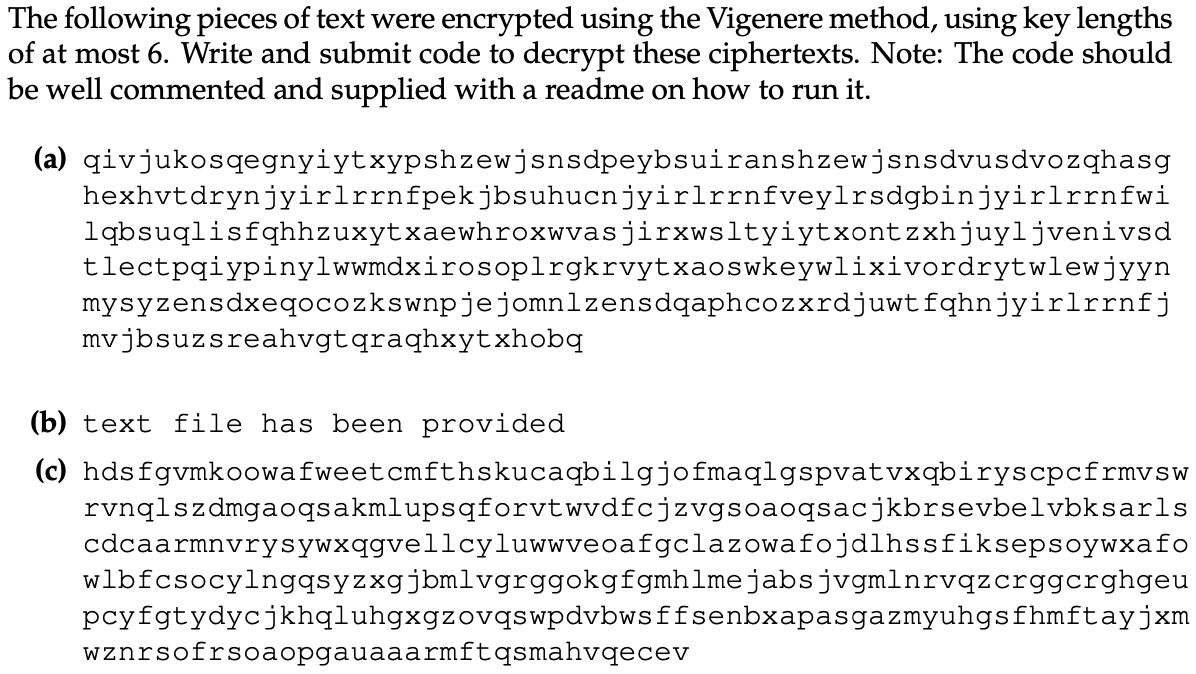
\includegraphics[width=17cm]{8}
\end{figure}

My code for decryption of the ciphertexts by using letter frequency analysis has been attached in:

\href{https://drive.google.com/drive/folders/1Pc5Ld6Vsz-CbPtESxMlKouj5Vsph8fID?usp=sharing}{Question 8}

(Also submitted on google classroom)

8.py covers the main code for the reference frequency table generation and decryption of the ciphertexts. The readme 8.md explains how to run my code. 8.ipynb shows my working for how I got my complete code. The building of the frequency table is covered more in 7/7.ipynb.

\clearpage
\section*{Problem 9 [10 points]}

\begin{figure}[h]
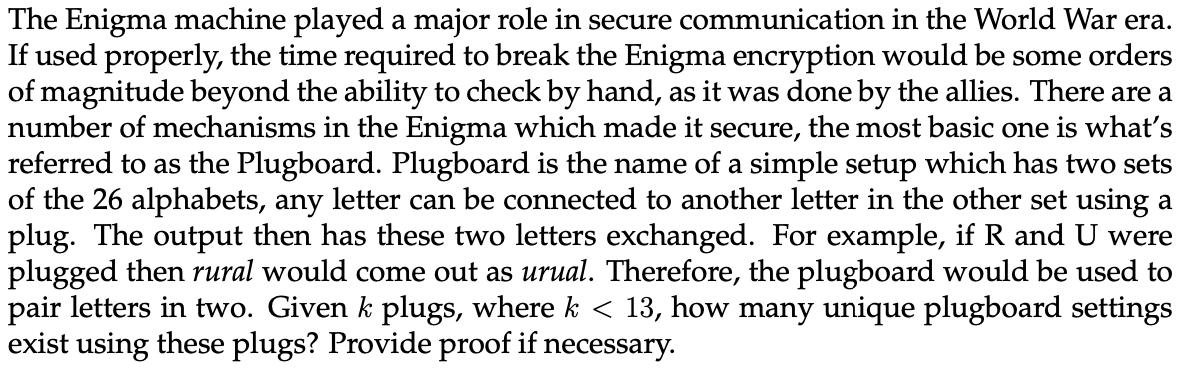
\includegraphics[width=17cm]{9}
\end{figure}

If there are $k$ plugs in plugboard, that is, there are groups of $13$ alphabets being considered in the two sets of the plugboard then the total number of alphabets selected from $26$ possible alphabets is $2k$.

The number of ways to select these $2k$ alphabets is:

\begin{math}
\binom{26}{2k} = \frac{26!}{26! \cdot (2k)!}
\end{math}

Now these $2k$ alphabets need to be divided into pairs. The first plug has $2k$ options, the second has $2k-1$ options, the third has $2k-2$ and so on until the last plugboard has 1 option.

Using the multiplication rule of counting,

The total possible pairs is $(2k)!$. 

This contains duplicate pairs as the order within a pair does not matter. So we divide this by $2^k$, as for each of the $k$ pairs there are $2$ orderings.

So $(2k)!/2^k$ gives us the total pair permutations possible without pair duplication.

We further divide this with $k!$ as the permutations of the $k$ pairs should not be counted,

$\frac{(2k)!}{2^k\cdot k!}$

Since, this is the total possible plugboard settings for each of the $\binom{26}{2k}$ selected alphabets, the total number of possible plugboard settings for each of $2k$ alphabet selections is,

\begin{math}
\binom{26}{2k}\cdot \frac{(2k)!}{2^k\cdot k!}
\end{math}

\end{document}

